
\documentclass[preprint,12pt]{elsarticle}
\makeatletter
\def\ps@pprintTitle{%
 \let\@oddhead\@empty
 \let\@evenhead\@empty
 \def\@oddfoot{\centerline{\thepage}}%
 \let\@evenfoot\@oddfoot}
\makeatother

\usepackage[spanish]{babel}
\usepackage{amssymb}
\usepackage{graphicx}
\usepackage{lineno}
\usepackage[utf8]{inputenc}
\usepackage{url}
\usepackage{natbib} 
\usepackage{amsmath} 
\usepackage{amssymb} 

\begin{document}
	\begin{frontmatter}
		\title{\huge Informe de Laboratorio 07 - Contenedor de Microsoft SQL Server}
		\author{Robles Flores, Anthony Richard              	(2016056192)}	
		\address{Universidad Privada de Tacna}
		\address{Escuela Profesional de Ingeniería de Sistemas}
		\address{Tacna, Perú}
	\end{frontmatter}

%% INFORMACIÓN GENERAL -----------------------------------------------------------------------------------------------------------------------------------
\section{INFORMACIÓN GENERAL}
Objetivos:
\begin{itemize}
\item Crear un contenedor de la imagen de Microsoft SQL Server 
\item Desplegar una BD usando un contenedor
\end{itemize}
Equipos y programas utilizados:
Para el siguiente laboratorio requerimos de:
\begin{itemize}
\item Computadora con sistema operativo Windows 10
\item Microsoft SQL Server Management Studio
\item Docker Desktop
\end{itemize}

%% MARCO TEORICO -----------------------------------------------------------------------------------------------------------------------------------
\section{MARCO TEÓRICO}
\begin{itemize}
\item Docker empaqueta software en “contenedores” que incluyen en ellos todo lo necesario para que dicho software se ejecute, incluidas librerías. Con Docker se puede implementar y ajustar la escala de aplicaciones de una forma rápida en cualquier entorno con la garantía de que el código se ejecutará.

A primera vista se piensa en Docker como una especie de máquina virtual liviana, pero la verdad no lo es. En Docker no existe un hypervisor que virtualice hardware sobre el cual corra un sistema operativo completo. En Docker lo que se hace es usar las funcionalidades del Kernel para encapsular un sistema, de esta forma el proyecto que corre dentro de el no tendrá conocimiento que está en un contenedor. Los contenedores se encuentran aislados entre sí y se comportaran como máquinas independientes.

Iniciar un contenedor no tiene un gran impacto a diferencia de iniciar una máquina virtual ya que no tiene que iniciar un sistema operativo completo (desde cero). Gracias al uso de contenedores la demanda de recursos baja limitándose sólo al consumo de la aplicación que contenga. Un contenedor inicia en milisegundos.
\item Anteriormente hablamos de manera de introducción sobre los contenedores pero ahora definamos en sí este concepto, Docker trabaja con algo que se llama contenedores de Linux estos son un conjunto de tecnologías que juntas forman un contenedor (de Docker), este conjunto de tecnologías se llaman:NamesSpace , Cgroups y Chroot.
\end{itemize}

%% PROCEDIMIENTO -----------------------------------------------------------------------------------------------------------------------------------
\section{PROCEDIMIENTO}
\textbf{Paso 1 : Iniciar Docker}
\begin{enumerate}[a)]
\item Iniciaremos con nuesytra cuenta docker en Docker Deskot.
\begin{figure}[htb]
	\begin{center}
		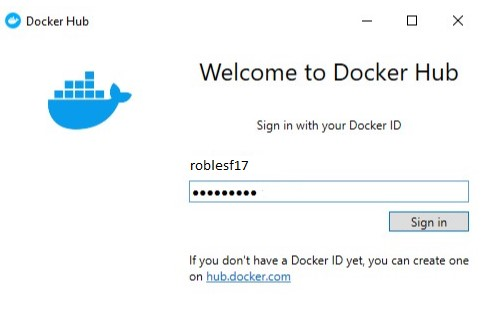
\includegraphics[width=8cm]{./IMAGENES/Docker01}
	\end{center}
\end{figure}
\item Debemos estar registrados para ingresar.
\item Ejecutamos PowerShell y agregamos el siguiente comando \textbf{docker version}.
\begin{figure}[htb]
	\begin{center}
		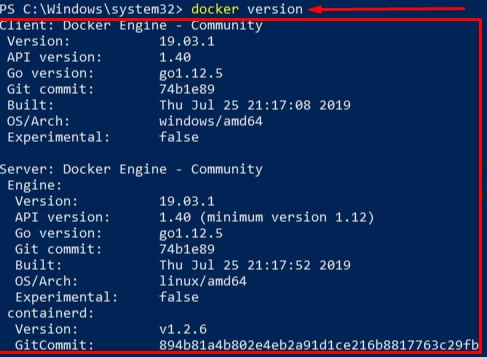
\includegraphics[width=6cm]{./IMAGENES/Docker02}
	\end{center}
\end{figure}


\textbf{Paso 2 : Crearemos un contenedor con Microsoft SQL Server para Linux}
\item Ejecutaremos el siguiente comando \textbf{docker search mssql} en PowerShell.
\begin{figure}[htb]
	\begin{center}
		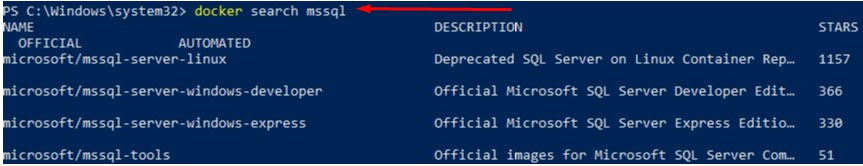
\includegraphics[width=11cm]{./IMAGENES/Docker03}
	\end{center}
\end{figure}
\item Ingraseremos nuestra cuenta en la página web Desktop Hub y buscaremos el repositorio \textbf{"microsoft/mssql-server-linux"}. 
\begin{figure}[htb]
	\begin{center}
		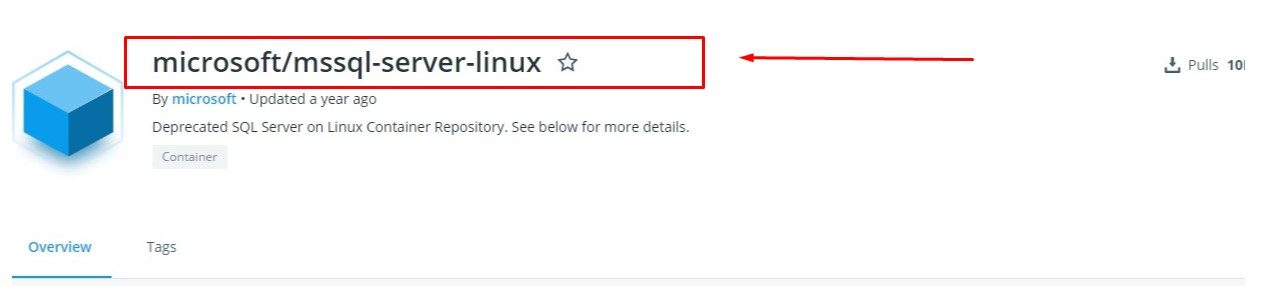
\includegraphics[width=9cm]{./IMAGENES/Docker04}
	\end{center}
\end{figure}
\item Copiando el comando en la aplicación PowerShell (docker pull microsoft/mssql-server-linux)
Se descargará la imagen del contenedor de Microsoft SQL Server en un servidor Linux como podemos ver en la imagen.
\begin{figure}[htb]
	\begin{center}
		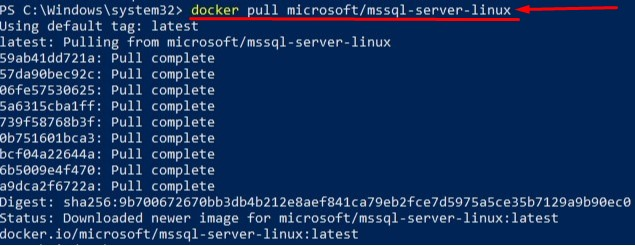
\includegraphics[width=11cm]{./IMAGENES/Docker05}
	\end{center}
\end{figure}


\item Verificaremos la imagen descargada con el siguiente comando \textbf{docker images}.
\begin{figure}[htb]
	\begin{center}
		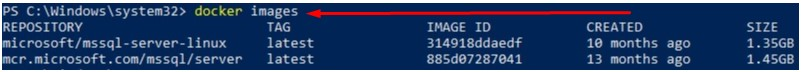
\includegraphics[width=14cm]{./IMAGENES/Docker06}
	\end{center}
\end{figure}

\item Iniciaremos el contenedor con el siguiente comando
\begin{figure}[htb]
	\begin{center}
		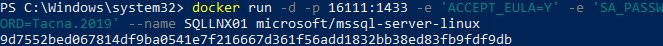
\includegraphics[width=14cm]{./IMAGENES/Docker07}
	\end{center}
\end{figure}

\item Nos devolcera el ID del contenedor.
\begin{center}
9d7552bed067814df9ba0541e7f216667d361f56add1832bb38ed83fb9fdf9db
\end{center}

\item Verificamos que el contenedor se está ejecutando correctamente con el siguiente comando docker ps. El resultado será similar al siguiente:
\begin{figure}[htb]
	\begin{center}
		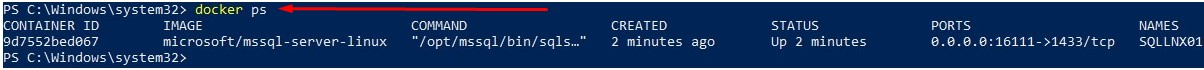
\includegraphics[width=14cm]{./IMAGENES/Docker08}
	\end{center}
\end{figure}

\item Abriremos el programa Microsoft SQL Server Management Studio 17 y conectamos con los siguientes datos: 
\begin{center}Nombre del servidor : 127.0.0.1,16111\end{center}
\begin{center} Inicio de sesión :sa\end{center}
\begin{center}Contraseña:Epis2019\end{center}
	\begin{figure}[htb]
		\begin{center}
		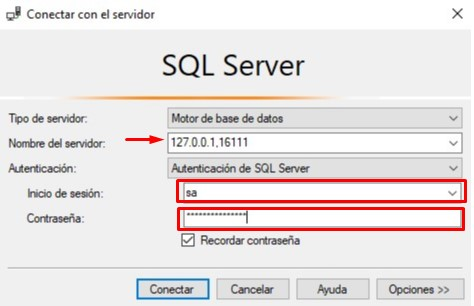
\includegraphics[width=9cm]{./IMAGENES/Docker13}
		\caption{Conectar con el Servidor}
		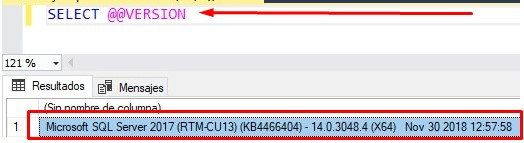
\includegraphics[width=8cm]{./IMAGENES/Docker11}
		\end{center}
	\end{figure}

\item Iniciaremos una consulta ingresando lo siguiente : 
\begin{center}SELECT @@VERSION\end{center}

\item En la aplicación PowerShell ejecutamos el siguiente comando:
\begin{center}docker rm -f SQLLNX01\end{center}
\item Verificamos la eliminación del contenedor con el siguiente comando:
\begin{center}docker ps\end{center}
\end{enumerate}

%% ANÁLISIS E INTERPRETACIÓN DE RESULTADOS -----------------------------------------------------------------------------------------------------------------------------------
\section{ANÁLISIS E INTERPRETACIÓN DE RESULTADOS}
\begin{enumerate}[a)]
\item Con el comando para iniciar con un contenedor podemos asignar los siguientes parámetros:
\begin{center} -p : 	Asignar el puerto.\end{center}
\begin{center}'sapassword' : Contraseña del Inicio de Sesion SQL, usuario sa.\end{center}
\begin{center} --name : Nombre del contenedor.\end{center}
\end{enumerate}


\section{CUESTIONARIO}

\begin{enumerate}[a)]
\item ¿Con qué comando(s) exportaría la imagen de Docker de Microsoft SQL Server a otra PC o servidor?\newline
Exportar la Imagen de Docker de Microsoft SQL Server
"docker export (ID contenedor) >  Nombreimagen.tar"
\begin{center} docker 9d7552bed067814df9ba0541e7f216667d361f56add1832bb38ed83fb9fdf9db > SQL.tar \end{center}
\begin{figure}[htb]
	\begin{center}
		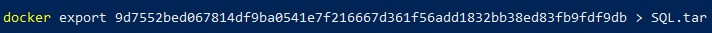
\includegraphics[width=14cm]{./IMAGENES/Docker17}
	\end{center}
\end{figure}
\item ¿Con qué comando(s) podría generar dos volúmenes para un contenedor para distribuir en un volumen el Archivo de Datos (.mdf) y en otro el Archivo Log (.ldf)?\newline
CREATE DATABASE NAMEDATABASE ON \newline
( FILENAME = N'/var/opt/mssql/data2/NDATABASE.mdf' ),\newline
( FILENAME = N'/var/opt/mssql/data2/NDATABASElog.ldf' )\newline
FOR ATTACH\newline
GO\newline
\item Genere un nuevo contenedor y cree la base de datos con las siguientes características.\newline
Nombre : FINANCIERA \newline
Archivos:
\begin{itemize}
\item DATOS (mdf) : Tamaño Inicial : 50MB, Incremento: 10MB, Ilimitado
\item INDICES (ndf) Tamaño Inicial : 100MB, Incremento: 20MB, Maximo: 1GB
\item HISTORICO (ndf) Tamaño Inicial : 100MB, Incremento: 50MB, Ilimitado
\item LOG (ldf) Tamaño Inicial : 10MB, Incremento: 10MB, Ilimitado
\end{itemize}
\item ¿Cuál sería el script SQL que generaría esta base de datos?
\begin{figure}[htb]
	\begin{center}
		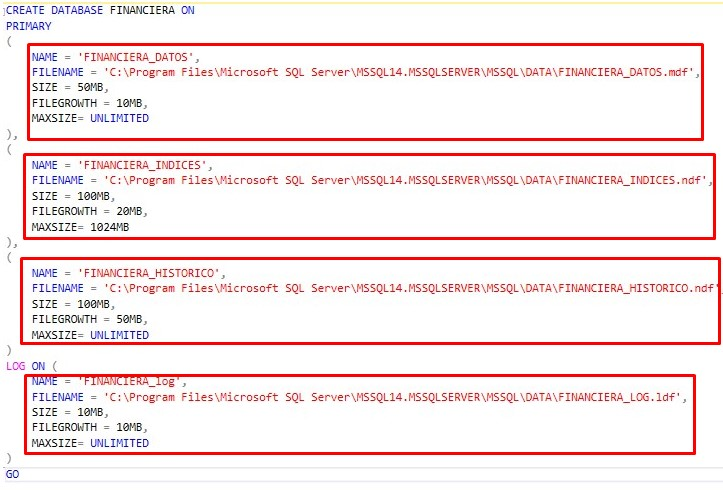
\includegraphics[width=10cm]{./IMAGENES/Docker14}
		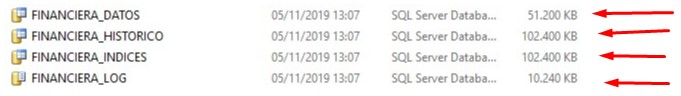
\includegraphics[width=10cm]{./IMAGENES/Docker15}
	\end{center}
\end{figure}
\end{enumerate}



\section{CONCLUSIONES}
Los contenedores de Docker nacen a partir de una imagen y en estos contenedores podemos solo ejecutar e instalar servicios, viene siendo como crear una maquina virtual a partir de una imagen (snapshot) pero muchísimo más ligera. 


\end{document}
